% ============ 5. Audit Results ============
\section{Audit Results}\label{sec:results}

\subsection{H1: baseline predictability under augmented inference}\label{sec:results:h1}

Table~\ref{tab:core} column (1) reports the pre-specified baseline: next-day close-to-close returns on named firm-day sentiment with controls, two-way clustered. The coefficient is $0.0149$ ($t=2.10$, $p=0.035$), i.e., a one-standard-deviation sentiment increase (0.36 on the $[-1,1]$ scale) is associated with a 54 \bps{} next-day return. Three augmentations discipline this number. First, the Rademacher wild-cluster bootstrap (day-level, null-imposed, $B=1{,}999$) gives $p=0.030$: the result is not an artifact of one or two trading days. Second, the Benjamini--Hochberg correction over the declared seven-comparison family raises the implied $q$-value to $0.062$: the headline baseline would not survive a 5\% FDR threshold. Third, adding the same-day return as a control~---motivated by the echo analysis below~---reduces the coefficient to $0.0141$ with $t=1.82$ ($p=0.069$); adding the overnight component as well gives $t=1.71$. The honest reading of H1 is \emph{marginal evidence, sensitive to specification, in a 205-observation sample}. The design's resolution is similarly bounded: at 80\% power, the minimum detectable next-day coefficient is $0.020$~---one-third larger than the estimate itself~---and the power of the test against the observed effect is $0.56$ (Appendix~\ref{app:power}).

For comparability with the literature, the same-day coefficient is $0.0283$ ($t=3.33$, $N=205$): sentiment co-moves with the return realized \emph{on} the news day. This co-movement is central to the echo analysis of Section~\ref{sec:results:h4}, which shows that the loading is a property of the text, not evidence about how prices form.

A final augmentation uses the full set of archived scoring draws of the same headlines: \emph{draw stability}. Re-estimating the identical H1 specification with every archived named draw~---fourteen independent passes plus the two within-condition means, spanning six sittings and both batch compositions (enumerated in Section~\ref{sec:robust})~---yields coefficients in $[0.0104,\,0.0161]$ and $t$-statistics in $[1.47,\,2.12]$, with both range endpoints set by individual passes (the October-16 single repeats individually run $t=2.12$, $1.76$, $1.68$). The point estimate is stable to well within its own standard error, but the \emph{nominal significance of H1 is draw-dependent}: the baseline draw sits at the favorable end of the range, and a pipeline that scored once on a different day would have reported $p$ between $0.05$ and $0.14$. We accordingly read H1 as \emph{borderline evidence with a stable point estimate}, which is exactly the resolution the power analysis of Appendix~\ref{app:power} predicts for a true effect of this size.

\begin{table}[htbp]
\centering
\small
\caption{Core audit regressions (dependent variable: next-day return unless noted)}
\label{tab:core}
\begin{threeparttable}
\begin{tabular}{lcccccc}
\toprule
 & (1) & (2) & (3) & (4) & (5) & (6) \\
 & Named & Named & Anon. & Dict. & Price-lang. & Clean \\
\midrule
Sentiment (named) & 0.0149$^{*}$ & 0.0141 & & & 0.0470 & 0.0033 \\
 & (2.10) & (1.82) & & & (1.80) & (0.61) \\
Sentiment (anonymized) & & & 0.0144 & & & \\
 & & & (1.78) & & & \\
Dictionary tone & & & & 0.0268 & & \\
 & & & & (1.00) & & \\
Same-day return & & 0.0306 & & & 0.0961 & $-$0.0211 \\
 & & (0.38) & & & (1.13) & ($-$0.29) \\
Controls & Yes & Yes & Yes & Yes & Yes & Yes \\
\midrule
$N$ & 205 & 205 & 205 & 205 & 38 & 167 \\
Wild-cluster bootstrap $p$ & 0.030 &~--- &~--- &~--- &~--- &~--- \\
BH family $q$ & 0.062 &~--- &~--- &~--- &~--- &~--- \\
\bottomrule
\end{tabular}
\begin{tablenotes}[flushleft]\footnotesize
\item All specifications include lagged return, lagged 21-day volatility, and the equal-weighted market return; $t$-statistics in parentheses, clustered by firm and trading day. Columns (5)--(6) split the sample by whether any headline for the firm-day contains realized-price language (15.2\% of headlines); both include the same-day return as a control. Wild-cluster bootstrap: Rademacher weights at the day level, null imposed, $B=1{,}999$. BH $q$: Benjamini--Hochberg FDR over the declared family of Table~\ref{tab:bh}. $^{*}$10\%, $^{**}$5\%, $^{***}$1\%.
\end{tablenotes}
\end{threeparttable}
\end{table}

Figure~\ref{fig:forest} presents all core coefficients with 95\% confidence intervals: the audit's message in one picture is that every instrument-condition coefficient is positive, every interval is wide, and the differences among them are the object of the next subsection.

\begin{figure}[htbp]
\centering
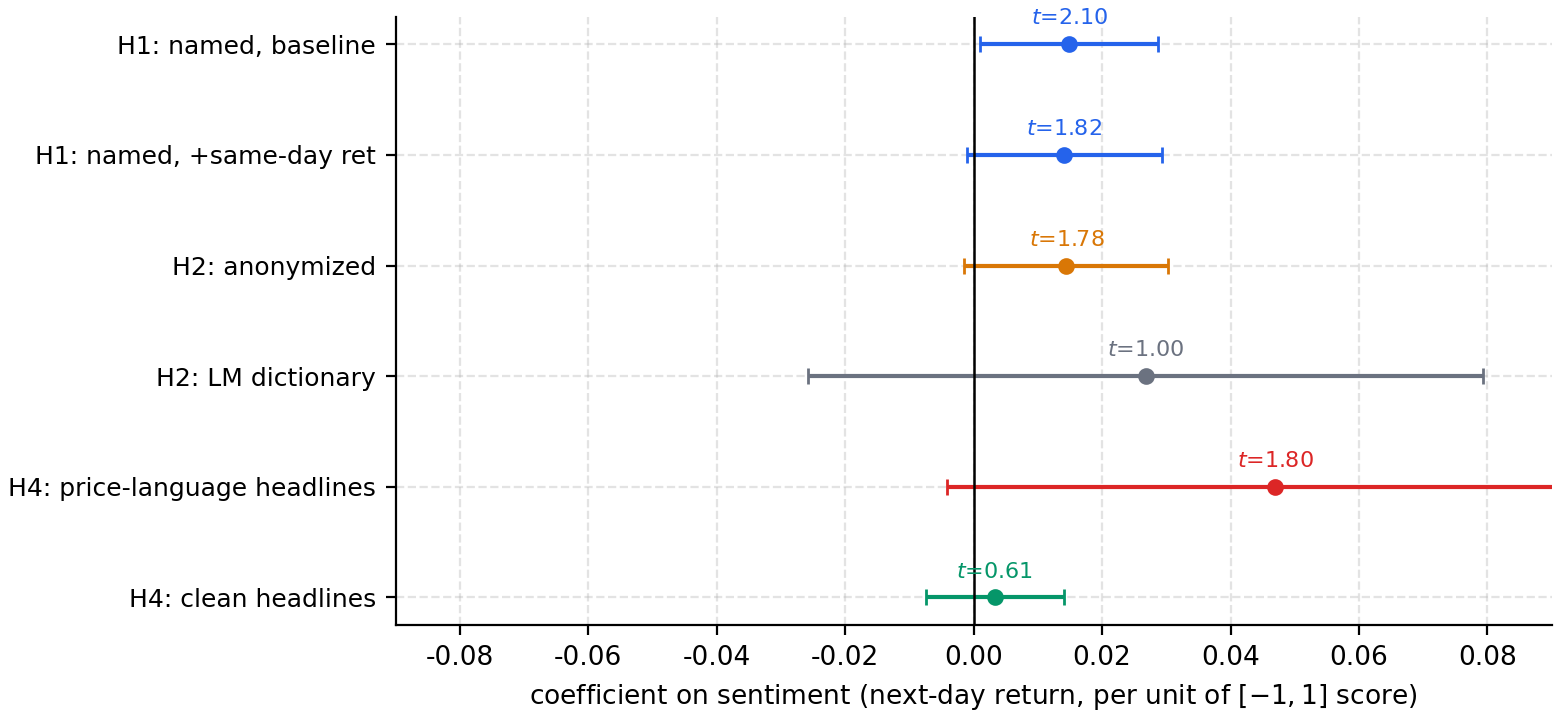
\includegraphics[width=0.92\textwidth]{../data/figures/fig_forest.png}
\caption{Core coefficients with 95\% confidence intervals (two-way clustered). No pairwise difference reaches conventional significance (Table~\ref{tab:diff}); the named, anonymized, and swapped conditions are formally equivalent at the half-benchmark margin, the dictionary comparison is inconclusive in both directions (Appendix~\ref{app:power}); the predictive loading is concentrated in price-language headlines.}
\label{fig:forest}
\end{figure}

\subsection{H2: de-identification shifts levels, not predictive content}\label{sec:results:h2}

\emph{The definitive estimate: a pre-specified, batch-interleaved design.} The identity contrast this paper reports was established by a third sitting (2026-10-18) that re-fielded both conditions under the protocol the audit ends up recommending: four rounds of the named protocol and four of the anonymized protocol over the identical 341 headlines, in a single sitting, with condition order alternated at the batch level (within each round, even-numbered batches of 25 call named-then-anonymized, odd-numbered call anonymized-then-named), protocol verbatim-identical, every call logged with timestamps and served-model identification (\texttt{glm-4-plus}). The design was pre-specified in an archived design document before any of its data was collected and is reported as a confirmatory contrast outside the declared family, well-powered under both headline-level and call-clustered inference. It establishes the identity level effect: $-2.82$ points in the named-minus-anonymized direction, with every one of the four round-level estimates negative ($-3.99$, $-2.05$, $-2.74$, $-2.51$; round-level $t=6.8$, $p=0.007$)~---\emph{anonymized scores sit systematically above their named twins by about three points}, a real but mild de-identification effect whose mechanism the fifth session's controls pin down below. One inference discipline applies here and below: because each API call returns all 25 scores of a batch in a single response, the scores of one call share a response-level \emph{mood} (Section~\ref{sec:results:h3} quantifies it at 13\% of residual variance), so headline-level paired tests overstate precision; under the most conservative clustering (14 batch-calls) the identity effect retains $t=2.7$ ($p=0.017$; 95\% CI $[-4.85, -0.79]$), and the estimate excluding the ten ticker-V headlines whose anonymization was a no-op (Appendix~\ref{app:anon}) is $-3.13$ with $t=4.8$ ($p=0.0003$). The order alternation makes call-order contamination testable: the effect is $3.34$ points (in the anonymized-minus-named direction) on batches where the named call came first versus $2.27$ where it came second~---similar magnitudes, no order artifact. The paired exact-match rate between interleaved condition calls is 48.5\%, bracketed by the within-condition repeat rates, exactly as a level displacement with stochastic noise predicts.

\emph{What the level effect is made of, and what it pools to.} A named-versus-anonymized contrast bundles two changes: the identity is removed, and the text is rewritten. Two pre-specified sittings separate the ingredients (2026-10-19 and 2026-10-25; design documents and falsifiable predictions archived before collection; Appendices~\ref{app:session5} and~\ref{app:session6}), and all contrasts below run under the locked analysis plans. \emph{Under corrected anonymization the contrast recurs}: with the ticker-V alias failure repaired and a forced verification pass reporting zero residual focal identifiers, the fifth sitting's named-minus-anonymized level difference is $-2.05$ points (headline-level $t=-2.84$, $p=0.005$; Wilcoxon $p<0.001$; under the conservative 14-cluster inference, $t=-1.36$, $p=0.18$), and the sixth sitting replicates it a third time (named minus anonymized $-2.54$, clustered $p=0.15$). Individually, only the interleaved session clears the conservative clustering, so the paper's summary number is the pooled one: across sessions 3, 5, and 6, a DerSimonian--Laird random-effects meta-analysis of the three call-clustered estimates ($-2.82$, SE 1.04; $-2.05$, SE 1.51; $-2.54$, SE 1.78) pools the de-identification effect at $-2.57$ points (95\% CI $[-4.08, -1.06]$, $z=3.34$; between-session heterogeneity nil: $\tau^2=0$, $I^2=0\%$). One caveat travels with the number: the three sessions re-score the same 341 headlines, and their per-headline responses correlate across sessions ($\rho=0.32$--$0.45$), so the three estimates are not independent draws; a conservative variant that adds those correlations to the full clustered standard errors widens the pooled interval to $[-4.56, -0.58]$~---still excluding zero (Appendix~\ref{app:session6}). \emph{The swap control does not support a material firm-specific prior}: replacing each headline's focal identifiers with a \emph{different} firm's identifiers~---natural text, wrong identity~---moves levels by $+0.34$ points against the named anchor ($t=0.40$, $p=0.69$; clustered $p=0.86$), far inside the repeat-noise floor, while the swapped condition sits $-2.39$ points below the anonymized one ($t=-3.26$, $p=0.001$; clustered $p=0.08$): the wrong firm's name sits with the right firm's name, two-plus points away from the placeholder. \emph{The prefix format is innocent}: adding a ``[Company X]'' prefix to the anonymized text moves levels by $+0.13$ (clustered $p=0.92$). \emph{A fictional-name control}~---scoring the identical 341 headlines with invented firm names, natural text, a concrete name, no real-world prior by construction~---places the fictional level almost exactly midway between named and anonymized (fictional minus named $+1.20$, clustered $p=0.45$; fictional minus anonymized $-1.33$, clustered $p=0.45$; the two clustered $p$-values are near-identical because the midpoint placement gives both sub-contrasts the same clustered $|t|$). Neither sub-contrast is individually established under clustered inference, so the split~---roughly half the displacement tied to the real name itself (identity associations or familiarity), half to the placeholder rewrite~---is a point-estimate reading rather than a certified decomposition. A leakage audit strengthens the swap contrast's reading: a transparent, data-driven cue lexicon flags 15.0\% of swapped headlines as still containing an original-firm lexical cue (26.7\% under a broader rule; six headlines, 1.8\%, retain the original identity outright through concatenated name variants such as ``ExxonMobil'' that the session-5 word-boundary verification cannot see), and excluding every flagged headline leaves the swap contrast at $+0.36$ to $+0.42$~---the null is not an artifact of identity leakage. The named-versus-anonymized level effect is therefore best read as a \emph{de-identification} effect~---removing the firm's real name raises scores, whoever the name belonged to~---with no support for a material prior about which firm the name denotes, and we use the accurate name throughout. The prediction layer agrees across every variant: the next-day coefficient is $0.0140$ (named), $0.0158$ (anonymized-v2), $0.0179$ (swapped), and $0.0134$ (prefixed; descriptive), with named-versus-anonymized and named-versus-swapped differences at $p=0.93$ and $p=0.92$~---de-identification moves levels, while the predictive coefficient stays formally equivalent at the half-benchmark margin. The formal level-layer equivalence battery at a pre-fixed margin of $\delta=1.25$ points (the prefix control certifies; the swap does not, minimum passing margin 1.73 points headline-level), the economics-anchored margins, and the session-by-session prediction-outcome tables are in Appendices~\ref{app:power}, \ref{app:session5}, and~\ref{app:session6}.


\emph{The superseded two-session benchmark.} The interleaved design exists because the original fielding~---named scores from 2026-10-15 against anonymized scores fielded twelve hours later~---read as a $+4.75$-point identity prior (paired $t=5.14$, $p<10^{-6}$), and the staged sessions then unraveled that reading: the named protocol itself drifted $+5.79$ points between the sittings, itself mostly batch composition, and the same-session residual~---a one-point displacement whose significance depended on the test and on the ticker-V exclusion~---was a range, not a verdict, which the interleaved design resolved at $-2.82$, opposite in sign to the naive shift. The full anatomy of the superseded benchmark~---distributional agreement, displacement magnitudes, the exact additive decomposition, the V-exclusion refinement, and the two figures that made the naive reading tempting~---is archived in Appendix~\ref{app:session} rather than carried in the main text, so the definitive interleaved estimate and its controls remain the only identity numbers a reader of the results must retain. The protocol lesson is general: condition contrasts fielded in separate sittings absorb session-level drift, and only same-session interleaving identifies the contrast the design intends.

\emph{What the drift is made of.} The interleaved session also closes the one question the two-session evidence could not answer: whether the $+5.79$ cross-session drift reflects the serving endpoint or the change in batch composition between sittings (session 1 scored the headlines embedded in the full 542-article stream; session 2 scored them alone). The October-18 sitting includes a control pass for exactly this: the \emph{identical} 341 headlines scored under the original 542-article batch composition, in the same session, same endpoint, same order. The composition effect is $+3.61$ points (headline-level paired $t=4.55$; batch-call-clustered $t=2.74$, $p=0.012$), and a fourth sitting re-ran the control with the run order \emph{inverted}~---composition pass first, 341-pass last, so that time-of-session works against the effect~---and reproduces it at $+3.50$ (clustered $t=2.17$); the pooled two-session estimate is $+3.56$ ($z=3.4$). Together with the two fixed-composition session legs, this gives an additive decomposition of the published drift: $+5.79 \approx +1.05$ (session 1 minus session 3, both at the 542 composition) $+\;3.61$ (composition, within session 3) $+\;1.14$ (session 3 minus session 2, both at the 341 composition), with the endpoint legs non-monotonic and the cross-session drift at fixed composition measuring $+0.56$ ($t=0.3$) between sessions 3 and 4. Batch composition, not endpoint change, carries roughly 62\% of the apparent ``session drift''~---which means the score of a headline depends measurably on \emph{which other headlines are scored alongside it}, a measurement-validity channel that, to our knowledge, has not previously been quantified in the LLM-finance setting; the NLP literature has documented the adjacent phenomena of batch-level accuracy loss and position/order sensitivity in batched prompting \citep{lin2024batch,liu2024lost,zheng2024}, but not their effect on the \emph{level} of a numeric measurement instrument. The fourth sitting also randomized the batch assignment of the 341 (seeded shuffle): re-batching the \emph{same} corpus moves levels by $+4.72$ points (clustered $t=2.02$, $p=0.065$~---suggestive). The mechanism accounting of Appendix~\ref{app:interleaved} bounds both shifts precisely, and neither lives in the linear part. Linear anchoring on batch-mates' fixed content is estimated at $\theta=+0.36$ ($t=4.9$; re-estimated with the full mate pool, $+0.38$, $t=5.0$), and for re-batching a \emph{fixed} corpus it \emph{provably} cannot shift the corpus mean (the telescoping identity: any re-partition preserves the average of leave-one-out batch-mate means). For the composition contrast the mate pool itself changes~---the 542-article batches seat each in-window headline next to out-of-window titles on 31\% of its batch-mate slots on average~---so there the linear component is quantifiable rather than barred: the 201 out-of-window titles average $-1.3$ points \emph{below} the in-window headlines they sit beside (35\% positive versus 62\%), and linear anchoring predicts a shift of $+0.04$ points against the observed $+3.56$~---about 1\%~---with full explanation requiring an out-minus-in content gap near $+30$ points, an order of magnitude beyond the actual gap and in the wrong direction. The estimated non-linearity does not close the residual either: asymmetric assimilation (positive batch-mates assimilate at $+0.69$, $t=2.3$; negative ones do nothing) would predict a small \emph{decrease}, because the added mates are less positive than those they replace. Both level shifts~---$+3.56$ from composition, $+4.72$ from re-batching alone~---therefore live almost entirely in response-level components that the current design does not separate: contrast-type responses to batch context, within-response position, and the mood shared by each response's 25 scores (Appendix~\ref{app:interleaved}, Table~\ref{tab:mech}). The mechanism is bounded, not closed, and we report it as such. A pre-registered batch-size dose-response session (a seeded 50-headline subsample scored alone, in fives, and in twenty-fives, one pass per size, within one sitting) leaves the presence channel open rather than closed: the singleton-versus-25 difference is $-0.20$ points ($t=-0.09$, $n=50$; SE $2.35$), so its 95\% CI of $[-4.92, +4.52]$ points cannot exclude a shift of the composition effect's own size~---an equivalence test would certify the singleton contrast only at a margin of $4.1$ points, wider than the effect itself~---and the same session carries an unexplained anomaly (the size-5 pass sits $5.5$--$5.7$ points below both neighbors, $t$ between $2.3$ and $2.5$) together with per-call noise SDs of 11--12 points across all three sizes that day, above the session-3 within-round benchmark of $7.2$ (Appendix~\ref{app:session6}). What the design establishes, under inverted run order, is that \emph{changed} mate composition moves levels; whether mere batch-mate presence also does is a question the dose-response leaves open. For pipelines the operational consequence is sharper than the session rule: hold the batch composition fixed across any comparison~---across conditions, sessions, or model versions~---because re-batching alone moves levels by more than the effect most studies are trying to measure.

\paragraph{Downstream consequences of the composition effect.} A natural objection: if levels move but slopes do not, what is the harm? The staged accounting over the archived sources of sessions 1--4 (all named protocol, identical 341 headlines; computed from archived draws, outside the declared family; \texttt{batch\_downstream.py}; full per-source accounting in Appendix~\ref{app:interleaved}) carries the operational verdict. Slopes and ranks are robust: the predictive coefficient stays in $[0.010, 0.016]$ across all seven sources, every composition and re-batch contrast of slopes is insignificant ($p>0.9$), and the cross-sectional ranking of firm-days correlates at $\rho\geq 0.81$ across compositions (0.97 at fixed composition across sessions). Absolute-scale uses are not robust: between the two compositions of the same session, a fixed ``score $\geq +50$'' filter more than doubles its trade count (22 to 50 firm-days in session 3; 27 to 43 in session 4), the daily-mean series shifts by 4.0--4.6 points, and the sign of the day-over-day change in daily sentiment flips on 16--24\% of trading days. The composition effect is therefore a \emph{level} pathology with boundary costs: harmless to conditional, cross-sectional, and regression uses in this sample, and disqualifying for threshold rules, absolute-score comparisons across pipelines, and time-series signals built on the score's level; Table~\ref{tab:downstream} and Figure~\ref{fig:downstream} itemize the accounting (Appendix~\ref{app:interleaved}).

\emph{Prediction layer.} The named-versus-anonymized predictive difference is tested three ways and never approaches significance: cross-session ($0.0004$, 95\% CI $[-0.0044, 0.0045]$, $p=0.887$), inside the October-16 sitting ($0.0002$, $p=0.905$), and interleaved inside October-18 ($+0.0013$, 95\% CI $[-0.0034, 0.0074]$, $p=0.622$)~---no difference is detected, which, as Section~\ref{sec:framework:inference} stresses, is not yet evidence of equivalence. Every instrument contrast is therefore re-assessed as a formal two-one-sided-tests (TOST) equivalence assessment at a margin of $\delta^{*}=0.0074$~---half the benchmark coefficient, about 27 \bps{} of next-day response per one-standard-deviation sentiment shock~---using the day-cluster bootstrap's 90\% interval as the test statistic and reporting each contrast's minimum passing margin so that any reader-preferred margin can be tested directly (Appendix~\ref{app:power}; exploratory, outside the declared family). The verdict upgrades some conclusions and bounds others. \emph{Upgraded}: all four named-versus-anonymized contrasts~---cross-session, same-session, interleaved, and the fifth session's corrected variant~---are formally equivalent at $\delta^{*}$, their 90\% intervals closing at 21--42\% of the benchmark coefficient (power 0.74--0.99 against a true difference of zero), so instrument invariance under de-identification is now an equivalence finding, not a failure to find. \emph{Bounded}: the swap contrast is the one near-miss~---its interval $[-0.0083, +0.0004]$ requires a margin of 0.0083, 56\% of the benchmark~---and the dictionary comparison is uninformative in \emph{both} directions: its interval $[-0.0658, +0.0415]$ fits no defensible margin ($4.4\times$ the benchmark, zero power, a hundredfold-plus sample needed), so this sample can establish neither that the LLM and the dictionary differ nor that they agree, and the earlier rhetorical question of which instrument ``wins'' is not answerable here. The verdicts are also margin-specific, and the benchmark-anchored margin is itself the weakest link~---the benchmark $t$ ranges over $[1.47, 2.12]$ across draws~---so Appendix~\ref{app:power} re-evaluates the battery at a stricter, economics-anchored margin of 10 \bps{} of next-day response per one-standard-deviation sentiment shock, a round threshold independent of the benchmark coefficient: no contrast passes (minimum passing margins run 11.5--29.8 \bps/SD across the four de-identification contrasts and the swap; the dictionary needs 237), and 3.6--7.8 times the sample would be required for 80\% power there, so the equivalence findings should be read as bounded at roughly a fifth to half of the benchmark effect rather than certified at arbitrary precision. The sixth session's prediction layer agrees across all three of its conditions ($\beta=0.0126$ named, $0.0112$ anonymized, $0.0113$ fictional; every pairwise difference $p\geq 0.62$). In a horse race on the same observations (not shown to avoid triple-counting), both coefficients remain individually insignificant at 5\%, which is exactly what low power plus attenuation predicts (Remark~\ref{prop:attenuation}, clause~(iii)).

\begin{table}[htbp]
\centering
\small
\caption{Formal difference tests (day-cluster bootstrap, $B=999$)}
\label{tab:diff}
\begin{threeparttable}
\begin{adjustbox}{max width=\textwidth}
\begin{tabular}{lccc}
\toprule
Contrast & Observed difference & 95\% CI & $p$-value \\
\midrule
$\beta_{\text{named}}-\beta_{\text{anonymized}}$ (cross-session) & 0.0004 & $[-0.0044,\ 0.0045]$ & 0.887 \\
$\beta_{\text{named}}-\beta_{\text{anonymized}}$ (same session) & 0.0002 & $[-0.0034,\ 0.0037]$ & 0.905 \\
$\beta_{\text{named}}-\beta_{\text{anonymized}}$ (interleaved) & 0.0013 & $[-0.0034,\ 0.0074]$ & 0.622 \\
$\beta_{\text{named}}-\beta_{\text{dictionary}}$ & $-$0.0119 & $[-0.0737,\ 0.0576]$ & 0.731 \\
$\beta_{\text{price-lang.}}-\beta_{\text{clean}}$ & 0.0436 & $[-0.0059,\ 0.1105]$ & 0.100 \\
Level shift, cross-session (points) & $+$4.75 &~--- & $<$0.0001 \\
Session drift (points) & $+$5.79 &~--- & $<$0.0001 \\
Identity, same session (points) & $-$1.04 & $[-2.32,\ +0.23]$ & 0.111 \\
Identity, same session, excl.\ V (points) & $-$1.29 & $[-2.53,\ -0.05]$ & 0.041 \\
Identity, interleaved sess.\ 3 (points) & $-$2.82 & $[-4.85,\ -0.79]$ & 0.017 \\
\quad excl.\ ticker V & $-$3.13 & $[-4.41,\ -1.86]$ & 0.0003 \\
De-identification, sess.\ 5, corrected anon.\ (points) & $-$2.05 &~--- & 0.175 \\
Identity swap vs.\ named, sess.\ 5 (points) & $+$0.34 &~--- & 0.857 \\
Composition effect, sess.\ 3 (points) & $+$3.61 & $[+1.03,\ +6.20]$ & 0.012 \\
Composition effect, sess.\ 4, order inverted & $+$3.50 &~--- & 0.042 \\
Re-batch (random), sess.\ 4 & $+$4.72 &~--- & 0.065 \\
Fictional minus named, sess.\ 6 (points) & $+$1.20 &~--- & 0.450 \\
Fictional minus anonymized, sess.\ 6 (points) & $-$1.33 &~--- & 0.450 \\
Identity (de-identification), sess.\ 6 (points) & $-$2.54 &~--- & 0.153 \\
Identity, pooled sess.\ 3/5/6, random effects & $-$2.57 & $[-4.08,\ -1.06]$ & 0.001 \\
Batch size 1 vs.\ 25, sess.\ 6b ($n=50$, points) & $-$0.20 & $[-4.92,\ +4.52]$ & 0.93 \\
\bottomrule
\end{tabular}
\end{adjustbox}
\begin{tablenotes}[flushleft]\footnotesize
\item Differences of next-day predictive coefficients from Table~\ref{tab:core} specifications; bootstrap resamples trading-day clusters ($B=999$; the price-language row uses $B=9{,}999$ under the same-day-control specification actually estimated, and is seed-stable: three independent seeds give $p$ between 0.093 and 0.100; the interleaved row uses $B=9{,}999$). Level rows are paired $t$-tests at the article level ($n=341$, points on the $[-100,100]$ scale): cross-session rows compare the 2026-10-15 named round with the 2026-10-16 round; the same-session identity rows compare the anonymized condition against the mean of the three October-16 named repeats. The last eight rows are staged confirmatory contrasts of the interleaved and control sessions (2026-10-18, a mechanism sitting, and 2026-10-19; Sections~\ref{sec:results:h2} and Appendix~\ref{app:interleaved}), each pre-specified in an archived design document before its data collection, reported outside the declared family, and evaluated under batch-call-clustered inference because the 25 scores of one API response share a response-level mood (13\% of residual variance; Section~\ref{sec:results:h3})~---headline-level tests of the same contrasts give $t=4.28$ (identity), $t=4.55$ (composition), and $t=-2.84$/$t=0.40$ (session-5 de-identification/swap), and the round-level identity meta-test gives $t=6.8$ ($p=0.007$). The V exclusion drops the ten headlines whose anonymization was a no-op (Appendix~\ref{app:anon}); the composition rows compare the identical 341 headlines scored inside the original 542-article batches versus the 341-only batches of the same session (session 4 with the run order inverted); the re-batch row compares seeded-random batches to the standard order. ``One significant, the other not'' never appears in this table by construction: all cross-instrument statements are direct difference tests. Computed by \texttt{analysis\_v2.py} (family rows), \texttt{revision\_power.py} and \texttt{v\_exclusion.py} (session rows), \texttt{analysis\_v3.py} / \texttt{analysis\_v4.py} / \texttt{reinference.py} (session-3/4 rows), and \texttt{analysis\_v5.py} (session-5 rows); the session-6 and batch-size rows are computed by \texttt{analysis\_v6.py} and \texttt{analysis\_v6b.py} under the same conventions (the batch-size row is a headline-level test on the 50-title subsample, where call clustering is degenerate), with level-layer equivalence margins from \texttt{level\_tost\_and\_margins.py} and the swapped-text leakage audit from \texttt{swap\_leakage\_audit.py} (Appendix~\ref{app:session6}). The pooled row is a DerSimonian--Laird random-effects meta-analysis of the three session-level clustered estimates, treating sessions as independent; because the sessions re-score the same 341 headlines, a conservative variant that applies the empirical cross-session correlation of per-headline responses ($\rho=0.32$--$0.45$) to the full clustered standard errors widens its interval to $[-4.56, -0.58]$ (\texttt{meta\_deident\_pooling.py}, \texttt{results\_meta\_deident.json}). The batch-size row's interval is the headline-level paired $t$ interval on the 50-title subsample.
\end{tablenotes}
\end{threeparttable}
\end{table}

The two-layer result is the paper's cleanest inference about what the model brings to the text~---corrected by its own staged designs and confirmed by the interleaved experiment, then re-attributed by the swap control: de-identification moves the level by $-2.6$ points pooled across three sessions (named scores sit \emph{below} their anonymized twins; the wrong firm's name sits with the right one), batch composition moves levels by another three-plus points, and the predictive signal they leave behind is formally equivalent at the half-benchmark margin in every de-identification contrast, with the swap contrast equivalent only at a 56\% margin (Appendix~\ref{app:power}). A displacement that raised all of a firm's headlines equally would be differenced out of any predictive regression that conditions on the firm; a displacement that differentially tracked which headlines \emph{matter} would have shown up as a predictive difference, and does not. The level evidence that initially pointed the other way measured the session and the batch, not the displacement~---and the sign it hid was the opposite of the naïve reading.

\subsection{H3: the instrument is reliable but stochastic}\label{sec:results:h3}

Four independent calls of the identical prompt on the identical headlines yield an intra-class correlation $\text{ICC}(2,4)=0.919$ with a bootstrap 95\% CI of $[0.90, 0.93]$; mean pairwise Pearson correlation across draws is $0.928$; 29.9\% of headlines receive the identical score in all four calls (44.0\% for the original-versus-draw-1 pair alone), and the mean within-headline standard deviation is 7.8 points (Figure~\ref{fig:reliability}). Those four calls span two sittings; the three October-16 draws alone give $\text{ICC}(2,3)=0.949$, so pooling across the twelve-hour gap costs three reliability points. The interleaved session answers the follow-up: Four October-18 named rounds give $\text{ICC}(2,4)=0.949$ with a within-headline standard deviation of 7.2 points (6.6 for the three October-16 rounds), and the interleaved anonymized rounds match (0.949): reliability is a stable property of the instrument, not of a particular sitting, even while the \emph{level} moves by points between the same sittings. The eight passes of the interleaved design also let the noise itself be decomposed, and the decomposition revises the intuition a single-repeat design encourages: 13\% of the residual variance is a \emph{response-level mood}~---a random level shared by all 25 headlines of one API response (SD $\approx2.6$ points)~---and only the remaining 87\% is idiosyncratic per headline per response (SD $\approx6.7$). Scoring is not 341 independent draws per pass but 14 correlated clusters, which is why the level contrasts of Section~\ref{sec:results:h2} are reported under call-clustered inference and why a pipeline that averages multi-headline batches inherits a noise floor its headline-level statistics hide. The pre-specified temperature-zero rounds of the fifth session close the loop on decoding settings: two identical named passes at \texttt{temperature}$\,=0$ return bitwise-identical scores for 83.3\% of headlines (284 of 341; within-headline SD 4.8 versus 7.2 under default decoding; mean absolute difference 2.4)~---substantially tighter, but 57 of 341 headlines still move between two calls at temperature zero, a pattern consistent with server-side nondeterminism that survives the decoding fix; the noise floor behaves as a property of the serving stack rather than of sampling settings alone. The temperature-zero level sits $+1.06$ points above the same-sitting default-decoding named level ($p=0.052$, two-sided, as pre-specified). The pooled number remains the right one for a production pipeline~---single-sitting ICCs overstate what re-scoring tomorrow will deliver~---which is also why the pooled ICC prices in the session drift of Section~\ref{sec:results:h2}. Reliability of $0.92$ is high by psychometric standards for a single-item instrument, and the mean-level agreement across draws (within one point) rules out gross instability. But it is emphatically \emph{not} determinism: a research pipeline that scores each headline once and treats the result as ``the'' score embeds a measurement-noise floor of $\pm8$ points per headline into every downstream construct. Under Remark~\ref{prop:attenuation}(i), the observed coefficient is attenuated by roughly the reliability ratio; with firm-day averaging over 1.25 headlines the attenuation is modest, which is the arithmetic reason the named and anonymized coefficients survive as similar point estimates. The practical implication is procedural: single-call scoring should report an ICC or repeat-call dispersion alongside any predictability statistic, and pipelines should score at least twice and average when headlines are cheap relative to inference~---as they are here.

\begin{figure}[htbp]
\centering
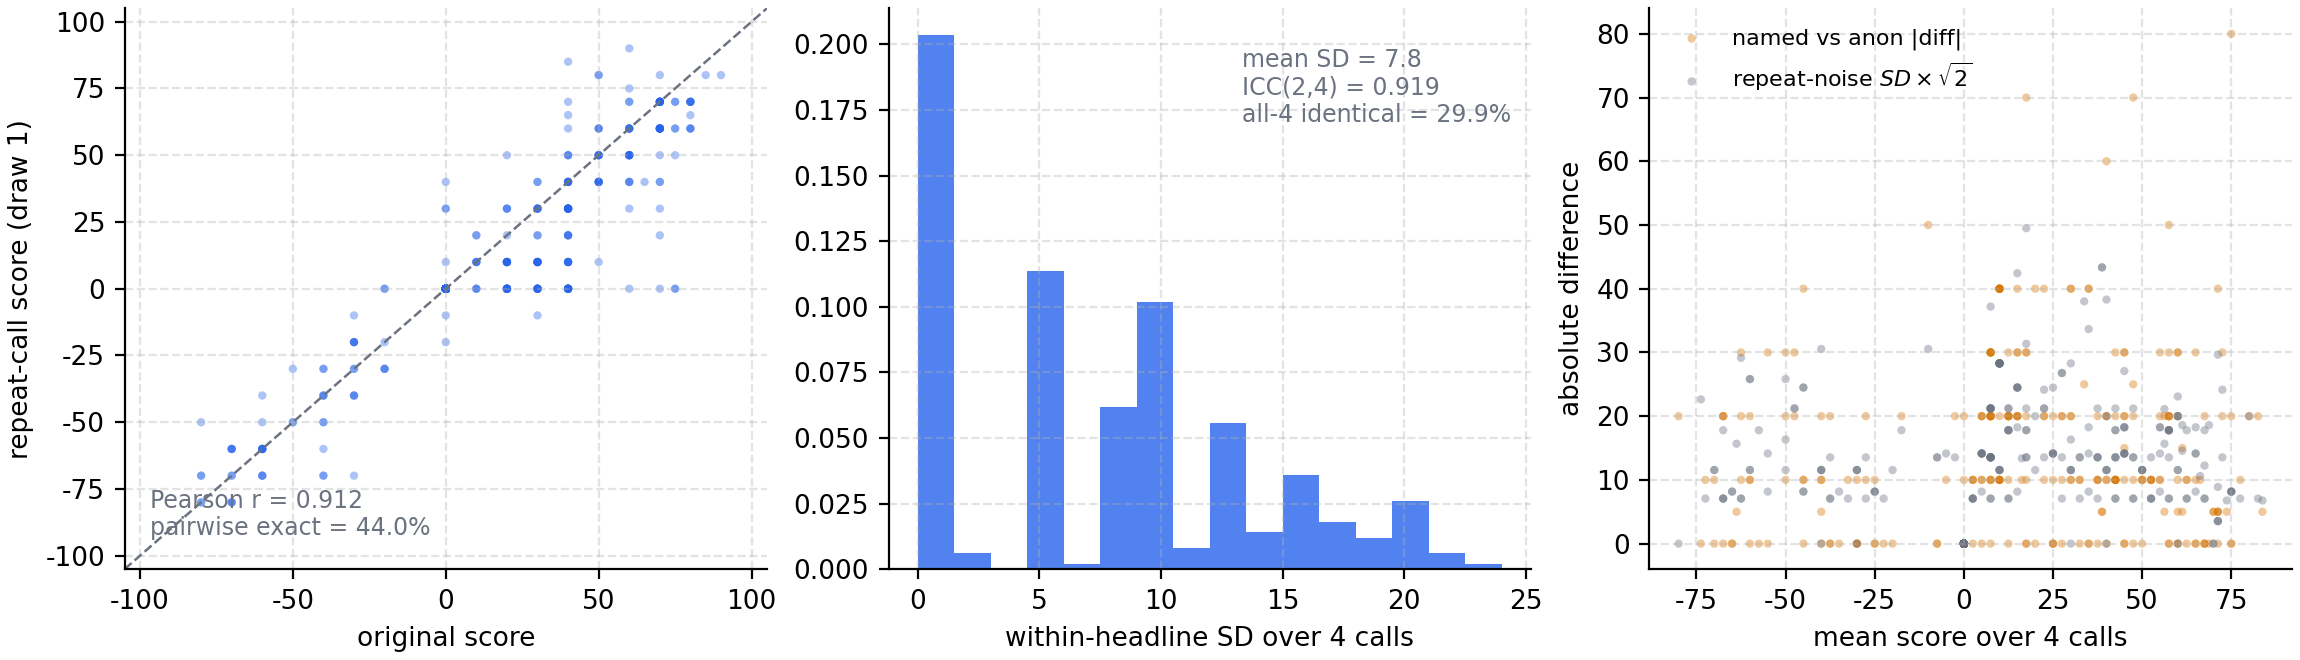
\includegraphics[width=\textwidth]{../data/figures/fig_reliability.png}
\caption{Repeat-call reliability. Left: original versus draw-1 scores ($r=0.912$; 44.0\% of the pair identical). Middle: within-headline standard deviation over four calls (mean 7.8 points); 29.9\% of headlines receive one identical score in all four calls. Right: Bland--Altman comparison of the named-versus-anonymized absolute difference against the repeat-noise floor ($\sqrt{2}\times$ within-SD): anonymization displaces scores by more than re-calling the model does.}
\label{fig:reliability}
\end{figure}

\subsection{H4: the predictive content sits in the price echo}\label{sec:results:h4}

A text audit flags headlines containing realized-price language~---movement verbs and magnitude constructions (``rose,'' ``surged,'' ``dropped by 5\% after earnings,'' ``up 20\% in 2026'')~---covering 52 of 341 in-window headlines (15.2\%). Table~\ref{tab:core} columns (5)--(6) split the firm-day sample by the flag (all specifications include the same-day return as a control): the coefficient is $0.047$ ($t=1.80$, $N=38$) for firm-days with price-language headlines and $0.003$ ($t=0.61$, $N=167$) without. The bootstrap difference is $0.044$ with 95\% CI $[-0.006, 0.110]$, $p=0.100$ ($B=9{,}999$, seed-stable; Table~\ref{tab:diff}): directional evidence~---underpowered in the tails and not clearing the 10\% threshold~---that the predictive loading concentrates where the text describes realized moves. On the magnitudes: the clean subsample's coefficient is one-fourteenth of the price-language coefficient ($0.003$ versus $0.047$) and about one-fifth of the baseline ($0.22$), insignificant~---but not established as \emph{equivalent} to zero: its 90\% interval reaches $0.0136$, 91\% of the benchmark (Appendix~\ref{app:power}), so this sample cannot separate ``no clean signal'' from ``a clean signal almost as large as the baseline.'' Essentially the entire point estimate of the baseline coefficient comes from the 19\% of the sample flagged as echoes.

Because the split's validity rests on a regular-expression classifier, we audited the classifier itself: all 52 flagged headlines were re-classified one by one against a written rulebook distinguishing realized price moves from fundamental-magnitude language, directional forecasts, and regex false positives. The classification is LLM-assisted and disclosed as such~---an internal audit of the flag, not independent human annotation (Appendix~\ref{app:classification}). The verdict: 43 of 52 (82.7\%) are genuine realized-price headlines, and re-running the split with only the strict realized-price firm-days leaves the point estimate essentially unchanged ($0.0475$ versus $0.0470$; $t=1.61$, $N=33$)~---the flag was noisy at the margin but not wrong where it mattered. The classification also sharpens the echo signature itself: strict-price firm-days average 361 \bps{} of absolute same-day return against 178 for clean days, while the nine misclassified headlines' firm-days average 120 \bps{}, below even the clean baseline. Leave-one-out and leave-one-company-out jackknifes of the priced-minus-clean difference keep every replicate positive (sign-flip rate 0.0; Appendix~\ref{app:classification}). The honest reading of H4 is unchanged by the audit~---directional, underpowered, text-located~---but it is now directional evidence whose classifier has itself been audited.

Two corroborating facts identify the channel as textual rather than mnemonic. First, the same-day loading of returns on sentiment is $t=3.33$ named and $t=3.11$ anonymized: if the same-day co-movement were driven by the scorer's memory of price outcomes, removing identity should have collapsed it; it barely moves. Second, the horizon path~---positive at $t+1$, negative at $t+2$ ($t=-2.04$)~---is exactly what short-horizon continuation-and-reversal around high-absolute-return events produces mechanically \citep{chan2003}, on a sample that (per H5) over-weights exactly those events. A reversal of this shape invites an attention-driven overshooting reading, but it is better read as the echo channel propagating through return dynamics; Section~\ref{sec:appaux} returns to this in the auxiliary analyses.

\begin{figure}[htbp]
\centering
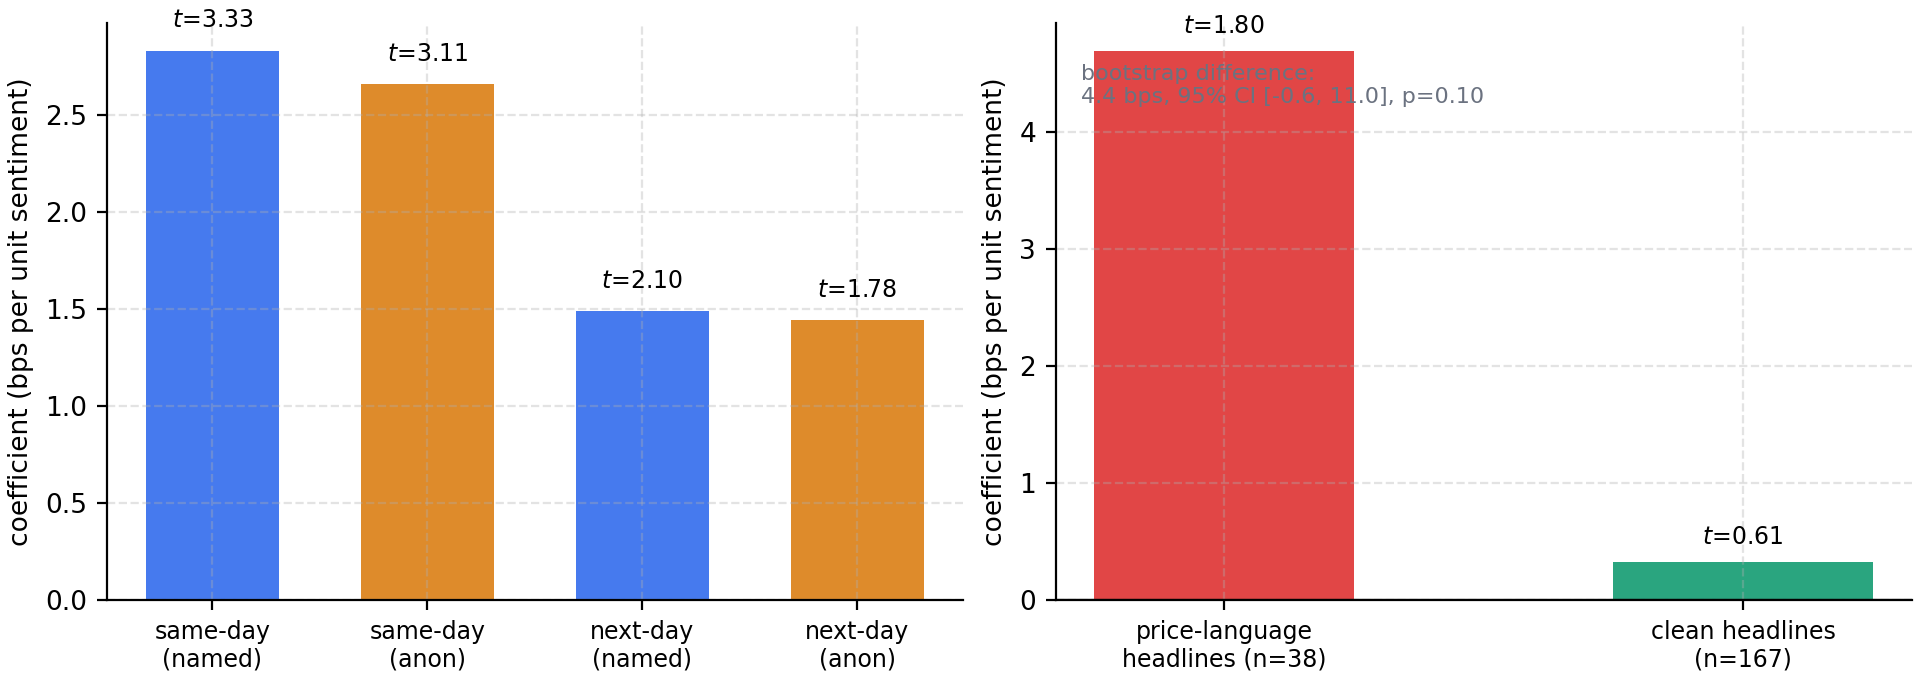
\includegraphics[width=\textwidth]{../data/figures/fig_echo.png}
\caption{The echo channel. Left: same-day and next-day coefficients, named versus anonymized~---anonymization does not remove the same-day loading (3.33 vs.\ 3.11), locating the contamination in the text. Right: next-day coefficients for price-language versus clean headlines, with the bootstrap difference.}
\label{fig:echo}
\end{figure}

\subsection{H5: coverage is selected on realized activity}\label{sec:results:h5}

Covered firm-days exhibit mean absolute same-day returns of 215 \bps{} against 154 \bps{} for uncovered firm-days, and firm-level news counts correlate 0.48 with firm return volatility (Figure~\ref{fig:selection}). A pooled two-sample statistic would pronounce this gap overwhelming ($t=3.12$, $p=0.002$), but it ignores the double indexing of the 2,664-cell panel~---the same firm repeats across days, and all firms share each trading day's market shock~---so the primary inference is a firm-and-day fixed-effects regression of absolute returns on the coverage indicator, estimated on the 2,628 firm-days with a non-missing same-day return (2,664 less the 36 first-trading-day cells, which lack a prior close), with two-way clustered standard errors: $t=2.76$ ($p=0.006$; BH $q=0.014$). Two robustness specifications agree: firm fixed effects with day-clustered errors give $t=2.49$ ($p=0.013$), and a day-cluster bootstrap of the gap gives $p\leq 0.002$ with 95\% CI $[25, 103]$ \bps. The selection equation~\eqref{eq:selection} is therefore rejected with $\delta_1>0$ under panel-appropriate inference: the audit sample over-weights high-activity events. It might be tempting to argue that coverage is driven by query design rather than by return outcomes, and that the consequence is statistical power rather than bias. That argument is wrong: search-driven collection selects on exactly the outcomes that make short-horizon continuation and reversal strongest for non-semantic reasons. The correction does not invalidate within-covered-sample inference, but it bounds external validity~---the estimand is the conditional (event-sampled) relationship, not the population relationship~---and it interacts with H4: high-activity events are both more likely to be covered and more likely to be covered \emph{retrospectively}.

\begin{figure}[htbp]
\centering
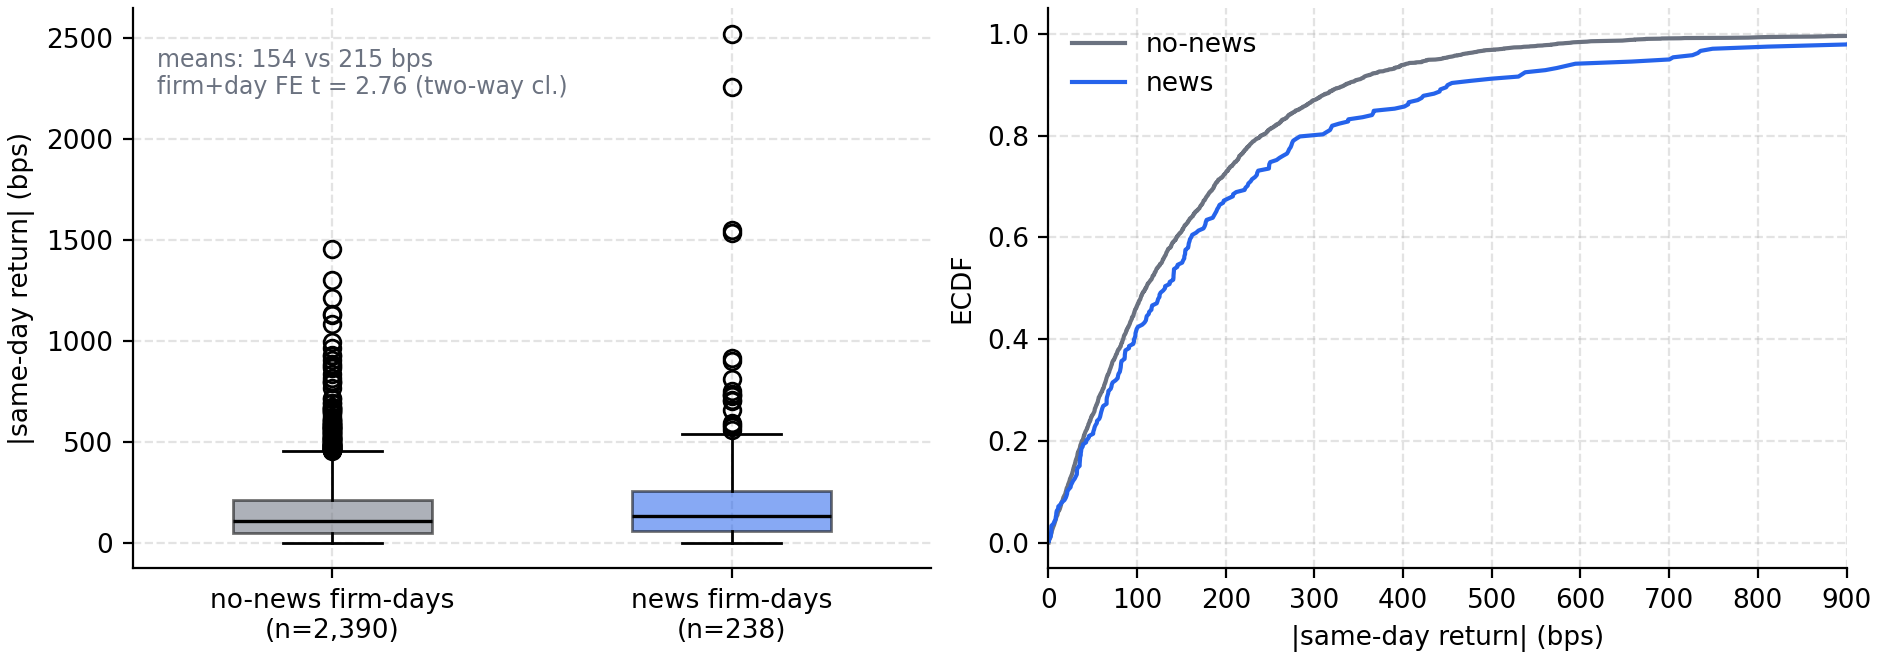
\includegraphics[width=0.95\textwidth]{../data/figures/fig_selection.png}
\caption{Coverage selection. Left: distribution of absolute same-day returns for covered versus uncovered firm-days. Right: empirical CDFs. Covered firm-days are drawn disproportionately from high-absolute-return states.}
\label{fig:selection}
\end{figure}

\subsection{Multiple-testing summary}

Table~\ref{tab:bh} reports the declared family with raw and Benjamini--Hochberg $q$-values. Three comparisons survive at any conventional threshold~---the named-versus-anonymized level shift ($q<0.0001$), the coverage-selection test ($q=0.014$), and the reliability ICC ($q<0.0001$, one-sided). The first of these requires re-interpretation rather than rejection: the level-shift test rejected because its contrast mixes an identity effect with a twelve-hour session gap, and the session component alone ($+5.79$, $t=7.03$) would clear any threshold; it survives as evidence of \emph{scoring instability across sittings}, not of an identity prior (Section~\ref{sec:results:h2}). The two channels that would constitute ``an LLM sentiment return signal''~---the baseline coefficient and its echo decomposition~---sit at $q=0.062$ and $q=0.140$ respectively. The pattern is itself informative: the audit finds the contamination and instability channels with confidence and the predictive content only marginally. The staged confirmatory contrasts of Section~\ref{sec:results:h2}~---the interleaved identity effect (round-level $p=0.007$; call-clustered $p=0.017$), its V-excluded variant ($p=0.0003$), the batch-composition effect (pooled $z=3.4$, two sessions with inverted run order), and the fifth session's swap and temperature-zero controls (Appendix~\ref{app:session5})~---sit outside the declared family by construction (they post-date it), but each was pre-specified in an archived design document before its data collection and they point the same way: the channels the audit measures with confidence are the ones the score carries for reasons other than the text's semantics.

\begin{table}[htbp]
\centering
\small
\caption{Declared test family: raw $p$-values and Benjamini--Hochberg $q$-values}
\label{tab:bh}
\begin{tabular}{lcc}
\toprule
Comparison & raw $p$ & BH $q$ \\
\midrule
H2: identity level shift (named $-$ anonymized) & $<$0.0001 & $<$0.0001 \\
H3: ICC $>$ 0.5 (one-sided bootstrap) & $<$0.0001 & $<$0.0001 \\
H5: coverage selection (firm+day FE, two-way cl.) & 0.0059 & 0.0137 \\
H1: baseline next-day coefficient (named) & 0.0354 & 0.0620 \\
H4: price-language vs.\ clean difference & 0.1002 & 0.1402 \\
H2: predictive difference, named vs.\ anonymized & 0.8869 & 0.8869 \\
H2: predictive difference, named vs.\ dictionary & 0.7307 & 0.8525 \\
\bottomrule
\end{tabular}
\begin{tablenotes}[flushleft]\footnotesize
\item Family declared in Section~\ref{sec:data} prior to augmented inference. The three rejections are measurement-layer channels; the two return-layer channels are marginal. $q$-values from the Benjamini--Hochberg step-up procedure at $m=7$. The H2 level-shift row compares conditions fielded twelve hours apart; Section~\ref{sec:results:h2} attributes most of it to between-session drift, and the same-session contrast ($p=0.11$, or $p=0.04$ excluding the ticker-V no-op anonymization) is a staged addition outside the declared family. The H5 row is the panel specification (firm and day fixed effects, two-way clustered; $N=2{,}628$ firm-days with non-missing same-day returns) that respects the panel's double indexing.
\end{tablenotes}
\end{table}
